\documentclass[twoside,a4paper]{article}
\usepackage{geometry}
\geometry{margin=1.5cm, vmargin={0pt,1cm}}
\setlength{\topmargin}{-1cm}
\setlength{\paperheight}{29.7cm}
\setlength{\textheight}{25.3cm}

% useful packages.
\usepackage{amsfonts}
\usepackage{amsmath}
\usepackage{amssymb}
\usepackage{amsthm}
\usepackage{enumerate}
\usepackage{graphicx}
\usepackage{multicol}
\usepackage{fancyhdr}
\usepackage{layout}
\usepackage{mathtools}

% some common command
\newcommand{\dif}{\mathrm{d}}
\newcommand{\avg}[1]{\left\langle #1 \right\rangle}
\newcommand{\difFrac}[2]{\frac{\dif #1}{\dif #2}}
\newcommand{\pdfFrac}[2]{\frac{\partial #1}{\partial #2}}
\newcommand{\OFL}{\mathrm{OFL}}
\newcommand{\UFL}{\mathrm{UFL}}
\newcommand{\fl}{\mathrm{fl}}
\newcommand{\op}{\odot}
\newcommand{\Eabs}{E_{\mathrm{abs}}}
\newcommand{\Erel}{E_{\mathrm{rel}}}

\begin{document}

\pagestyle{fancy}
\fancyhead{}
\lhead{Jovi Wong(3180104829)}
\chead{Numerical Analysis homework \#04}
\rhead{2020/4/10}


\section*{I. Determine $p \in \mathbb{P}_3$}
We can suppose
\[
p(x)=a_1x^3+a_2x^2+a_3x
\]
Because $s(x)\in \mathbb{C}^2[0,2]$, then $p$ and $s$ derivatives are equal at $x=1$ 
\[
\left\{\begin{lgathered}
a_1+a_2+a_3=1 \\
3a_1+2a_2+a_3=-3\\
6a_1+2a_2=6 \\
\end{lgathered} \right. 
\]
We can get these coefficients easily, that is 
\[
\left\{\begin{lgathered}
a_1=7\\
a_2=-18\\
a_3=12 \\
\end{lgathered} \right. 
\]
Namely, $p(x)=7x^3-18x^2+12x$ , where $x\in[0,1]$. Functiion $s(x)$ isn't a natrual cubic spline since $p''(0)=-36$ .

\section*{II. Interpolating $f$ on $[a,b]$ with a quadratic spline $s\in\mathbb{P}_2^1$}
\subsection*{a.Why an additional condition is needed to determine $s$ uniquely}
We can suppose $p(x)=a_1x^2+a_2x+a_3$ where $x\in[x_i,x_{i+1}]$ and $a_1\neq0$, $\forall i\in\{1,2,\cdots,n-1\}$ . There are three coefficients, howerever, only can get two equations
\[
\left\{
\begin{lgathered}
a_1x_i^2+a_2x_i+a_3=f_i\\
a_1x_{i+1}^2+a_2x_{i+1}+a_3=f_{i+1}
\end{lgathered} 
\right.
\]
according to given conditions. So $s$ can't be determined uniquely.
\subsection*{b.determine $p_i$ and $m_i$}
Suppose $p_i(x)=a_1(x-x_i)^2+a_2(x-x_i)+f_i$ where $x \in [x_i,x_{i+1}]$, then
\[
\left\{
\begin{lgathered}
a_1(x_{i+1}-x_i)^2+a_2(x_{i+1}-x_i)+f_i=f_{i+1}\\
a_2=m_i
\end{lgathered} 
\right.
\]
We cat get the explicit coefficient by solving linear equations
\[
p_i(x)=\frac{f[x_i,x_{i+1}]-m_i}{x_{i+1}-x_i}(x-x_i)^2+m_i(x-x_i)+f_i
\]

\subsection*{c.show how $m_i$ can be computed}
The the first-order derivative of $p_i(x)$ is 
\[
p_i'(x)=2a_1(x-x_i)+a_2
\]
If $m_{i}=p'_{i}(x_i)$, we can know the answer recursively
\[
m_{i+1}=m_i+2\frac{f[x_i,x_{i+1}]-m_i}{x_{i+1}-x_i}
\]
\section*{III. Determine $s_2(x)$ on $[-1,1]$ and how to chose $c$ such that $s(1)=-1$}
Suppose $s_2(x)=a_1x^3+a_2x^2+a_3x+(1+c)$. It is obvious that $s'_1(0)=3c$ , $s''_1(0)=6c$ and $s''_2(1)=0$, then
\[
\left\{
\begin{lgathered}
a_1=-c\\
a_2=3c\\
a_3=3c\\
\end{lgathered} 
\right.
\]
since $s(x)\in \mathbb{P}_3^2$. Namely, $s_2(x)=-cx^3+3cx^2+3cx+(1+c)$. If $s(1)=-1$, it implies $c=-\frac{1}{3}$ .
\section*{IV.Consider $f(x)=\cos{(\frac{\pi}{2}x})$ with $x\in[-1,1]$}
\subsection*{a.determine natrual cubic spline on knots $-1,0,1$}
Suppose $p_1(x)=a_1(x+1)^3+a_2(x+1)^2+a_3(x+1)$ , where $x \in [-1,0]$. Since $p_1$ is a natrual cubic spline, $p''_1(-1)=0$ , $p_1(0)=f(0)$ , then take them into $p_1$ and we get
\[
\left\{
\begin{lgathered}
a_1+a_2+a_3=1\\
a_2=0\\
\end{lgathered} 
\right.
\]
So we can rewrite $p_1$ as $p_1(x)=a_1(x+1)^3+(1-a_1)(x+1)$ , where $x\in[-1,0]$.  Similarly, on $[0,1]$ , suppose 
\[
p_2(x)=b_1(x-1)^3+b_2(x-1)^2+b_3(x-1)
\]
Through $p''_2(1)=0$ and $p_2(0)=1$, we can get
\[
\left\{
\begin{lgathered}
b_2=0\\
b_1+b_2+b_3=-1
\end{lgathered} 
\right.
\]
Namely, $p_2(x)=b_1(x-1)^3-(b_1+1)(x-1)$.\\
\\
Function $s(x)$ must satisfy $p'_1(0)=p'_2(0)$ and $p''_1(0)=p''_2(0)$, so we can know
\[
\left\{
\begin{lgathered}
a_1+1=b_1\\
a_1=-b_1
\end{lgathered} 
\right.
\]
Consequently, $a_1=-\frac{1}{2}$ and $b_1=\frac{1}{2}$ . Take them into $s(x)$,
\[\text{s(x)=}
\left\{
\begin{lgathered}
-\frac{1}{2}(x+1)^3+\frac{3}{2}(x+1) , x \in [-1,0]\\
\frac{1}{2}(x-1)^3-\frac{3}{2}(x-1) , x \in [0,1]
\end{lgathered} 
\right.
\]
\subsection*{b.verify natural cubic splines have the minimal total bending energy}
We can get the second-order derivatives of $s(x)$ from the discussion above
\[\text{$s''(x)=$}
\left\{
\begin{lgathered}
-3(x+1) , x \in [-1,0]\\
3(x-1) , x \in [0,1]
\end{lgathered} 
\right.
\]

So it is obvious that
\begin{gather}
\int_{-1}^1[s''(x)]^2 \dif x=6
\end{gather}
\\
(1) When $g(x)=-x^2+1$, $g''(x)=-2$ , we can conclude
\begin{gather}
\int_{-1}^1[s''(x)]^2 \dif x < \int_{-1}^1[g''(x)]^2 \dif x=8 
\end{gather}
(2) When $g(x)=\cos{(\frac{\pi}{2}x)}$, $g''(x)=-\frac{\pi^2}{4}\cos{(\frac{\pi}{2}x)}$ , we can conclude
\begin{gather}
\int_{-1}^1[s''(x)]^2 \dif x < \int_{-1}^1[g''(x)]^2 \dif x= \frac{\pi^4}{16} 
\end{gather}
\section*{V.The quadratic B-spline $B_i^2(x)$}
\subsection*{a.derive the expression of $B_i^2(x)$}
According to definition 4.28 and example 4.7,
\[\text{$B_i^1(x)=$}
\left\{
\begin{lgathered}
\frac{x-t_{i-1}}{t_i-t_{i-1}}, x \in (t_{i-1},t_i]\\
\frac{t_{i+1}-x}{t_{i+1}-t_i}, x\in (t_i,t_{i+1}]
\end{lgathered} 
\right.
\]
\[\text{$B_{i+1}^1(x)=$}
\left\{
\begin{lgathered}
\frac{x-t_{i}}{t_{i+1}-t_i}, x \in (t_i,t_{i+1}]\\
\frac{t_{i+2}-x}{t_{i+2}-t_{i+1}}, x\in (t_{i+1},t_{i+2}]
\end{lgathered} 
\right.
\]
\begin{gather}
B_i^{2}(x)=\frac{x-t_{i-1}}{t_{i+1}-t_{i-1}}B^1_i(x)+\frac{t_{i+2}-x}{t_{i+2}-t_i}B_{i+1}^1(x)
\end{gather}
So we can easily get the answer,
\[\text{$B_{i}^2(x)=$}
\left\{
\begin{lgathered}
\frac{(x-t_{i-1})^2}{(t_{i+1}-t_{i-1})(t_i-t_{i-1})},\qquad\qquad\qquad\qquad\qquad\qquad x \in (t_{i-1},t_{i}]\\
\frac{(x-t_{i-1})(t_{i+1}-x)}{(t_{i+1}-t_{i-1})(t_{i+1}-t_i)}+\frac{(x-t_i)(t_{i+2}-x)}{(t_{i+2}-t_i)(t_{i+1}-t_i)}, \ \ \quad x\in (t_{i},t_{i+1}]\\
\frac{(t_{i+2}-x)^2}{(t_{i+2}-t_i)(t_{i+2}-t_{i+1})}, \qquad \qquad\qquad \qquad\qquad\qquad x \in (t_{i+1},t_{i+2}]\\
0, \qquad \qquad\qquad\qquad\qquad\qquad\qquad\qquad\qquad\qquad\quad \  otherwise
\end{lgathered} 
\right.
\]
\subsection*{b.verify $\frac{d}{dx}B_i^2(x)$ is continuous at $t_i$ and $t_{i+1}$}
From the explicit expression of $B_i^2(x)$, we can get its derivative
\[\text{$\frac{\dif}{\dif x} B_i^2(x)=$}
\left\{
\begin{lgathered}
\frac{2x-2t_{i-1}}{(t_{i+1}-t_{i-1})(t_i-t_{i-1})},\qquad\qquad\qquad\qquad\qquad\quad x \in (t_{i-1},t_{i}]\\
\frac{-2x+t_{i-1}+t_{i+1}}{(t_{i+1}-t_{i-1})(t_{i+1}-t_i)}+\frac{-2x+t_i+t_{i+2}}{(t_{i+2}-t_i)(t_{i+1}-t_i)},\ \ x\in (t_{i},t_{i+1}]\\
\frac{2x-2t_{i+2}}{(t_{i+2}-t_i)(t_{i+2}-t_{i+1})}, \qquad \qquad\qquad\qquad\qquad\quad x \in (t_{i+1},t_{i+2}]\\
0, \qquad\qquad\qquad\qquad\qquad\qquad\qquad\qquad\qquad\qquad \ otherwise
\end{lgathered} 
\right.
\]
Therefore,
\begin{gather}
\frac{\dif}{\dif x} B_i^2(t_i)=\frac{2t_i-2t_{i-1}}{(t_{i+1}-t_{i-1})(t_i-t_{i-1})}=\frac{-2t_i+t_{i-1}+t_{i+1}}{(t_{i+1}-t_{i-1})(t_{i+1}-t_i)}+\frac{-t_i+t_{i+2}}{(t_{i+2}-t_i)(t_{i+1}-t_i)}=\frac{2}{t_{i+1}-t_{i-1}}\\
\frac{\dif}{\dif x} B_i^2(t_{i+1})=\frac{t_{i-1}-t_{i+1}}{(t_{i+1}-t_{i-1})(t_{i+1}-t_i)}+\frac{-2t_{i+1}+t_i+t_{i+2}}{(t_{i+2}-t_i)(t_{i+1}-t_i)}=\frac{2t_{i+1}-2t_{i+2}}{(t_{i+2}-t_i)(t_{i+2}-t_{i+1})}=\frac{2}{t_i-t_{i+2}}
\end{gather}
Hence, $\frac{\dif}{\dif x}B_i^2(x)$ is continuous at $x=t_i$ and $x=t_{i+1}$ .
\subsection*{c.show that only one $x^* \in(t_{i-1},t_{i+1})$ satisfies $\frac{d}{dx}B_i^2(x^*)=0$}
Notice that $\frac{\dif}{\dif x} B_i^2(t_{i-1})=0$ and $\frac{\dif}{\dif x} B_i^2(x)$ increases on $(t_{i-1},t_i]$ strictly, so there is no zero of  $\frac{\dif}{\dif x} B_i^2(x)$ in this interval. \\ \\As for $(t_i,t_{i+1}]$, $\frac{\dif}{\dif x} B_i^2(x)$ decreases on this interval
strictly. Besides, $\frac{\dif}{\dif x} B_i^2(t_i)=\frac{2}{t_{i+1}-t_{i-1}}>0$ and $\frac{2}{t_{i}-t_{i+2}<0}$,\\ \\which indicates that $x^*=\frac{t_{i+1}t_{i+2}-t_{i-1}t_i}{t_{i+2}+t_{i+1}-t_{i-1}-t_i}$ is the unique zero of $\frac{\dif}{\dif x} B_i^2(x)=0$ .
\subsection*{d.show $B_i^2(x) \in [0,1)$}
From the discussion aboove, we know $\frac{\dif}{\dif x} B_i^2(x)$ increases on $[t_{i-1},x^*]$ and decreases on $[x^*,t_{i+2}]$, so 
\begin{gather}
\min{B_i^2(x)}=\min{\{B_i^2(t_i),B_i^2(t_{i+2})\}} = 0\\
\max{B_i^2(x)}=B_i^2(x^*)=\frac{t_{i+2}-t_{i-1}}{t_{i+2}+t_{i+1}-t_{i-1}-t_i}<\frac{t_{i+2}-t_{i-1}}{t_{i+2}-t_{t-1}}=1
\end{gather}
Hence, $0 \leq B_i^2(x) \leq B_i^2(x^*)<1$, namely , $B_i^2(x) \in [0,1)$ has proved.
\subsection*{e.Plot $B_1^2(x)$ for $t_i=i$}
$\\
\\
\\
$
\begin{figure}[h]
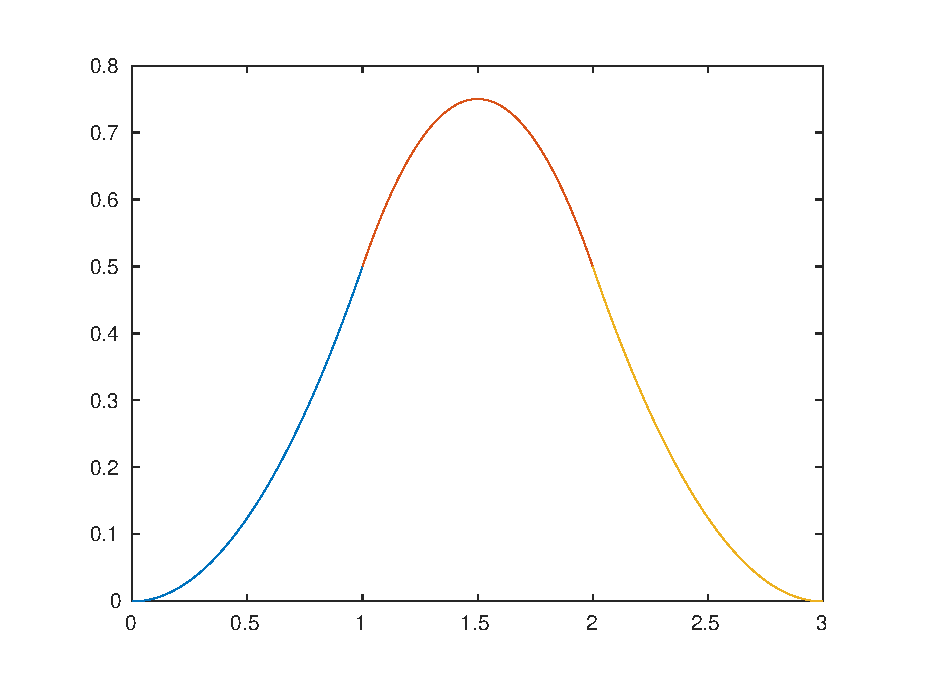
\includegraphics[width=7in]{b12(x).eps}
 \caption{$B_1^2(x)$}
\end{figure}

\section*{VI.Verify Theorem 4.23 in case of $n=2$}
Definition 4.18 and the Example 4.10 yield
\begin{gather}
B^2_1(x)=\beta(x)+\gamma(x)\\
B_i^1(x)=(t_{i+1}-t_{t-1})[t_{i-1},t_{i},t_{i+1}](t-x)_+\\
B_{i+1}^1(x)=(t_{i+2}-t_{t})[t_{i},t_{i},t_{i+2}](t-x)_+
\end{gather}
where,
\begin{gather}
\beta(x)=\frac{x-t_{i-1}}{t_{i+1}-t_{i-1}}B_i^1(x)=[t_i,t_{i+1}](t-x)_{+}^1-[t_{i-1},t_i,t_{i+1}](t-x)_{+}^{2}\\
\gamma(x)=\frac{t_{n+2}-x}{t_{n+2}-t_i}B_{i+1}^1(x)=[t_i,t_{i+1},t_{i+2}](t-x)^2_{+}-[t_i,t_{i+1}](t-x)_+^1
\end{gather}
Therefore,
\begin{gather}
B^2_1(x)=[t_i,t_{i+1},t_{i+2}](t-x)_{+}^{2}-[t_{i-1},t_{i},t_{i+1}](t-x)_{+}^{2}\\
=(t_{i+2}-t_{i-1})[t_{i-1},t_i,t_{i+1},t_{i+2}](t-x)_+^2
\end{gather}
Hence proved.
\\

\section*{Programming}
From the picture below, Runge phenomenon doesn't appear when we utilize cubic splines to approch the original function $ f(x)=\frac{1}{1+25x^2}$


\begin{figure}[h]
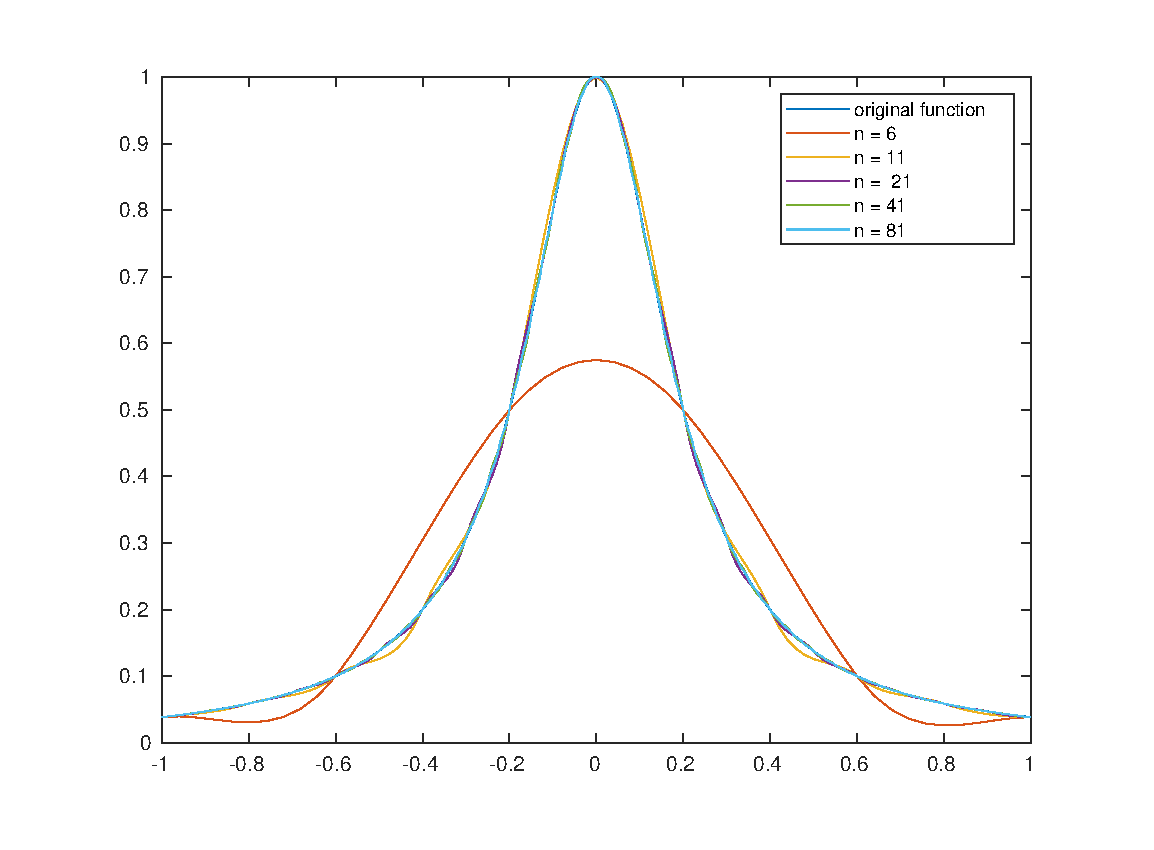
\includegraphics[width=7in]{cubic_splines.eps}
 \caption{cubic splines}
\end{figure}
Besides, the errors at each sampling points are as following as Figure 3 and Figure 4. To
be specific, error varies extremely depending on $N$, so Figure 3 is overall situation and Figure 4 is the situation near $x=0$ . These figures will present the max-norm of interpoloting errors clearly. From the the rate of convergence is really quick 

\begin{figure}[h]
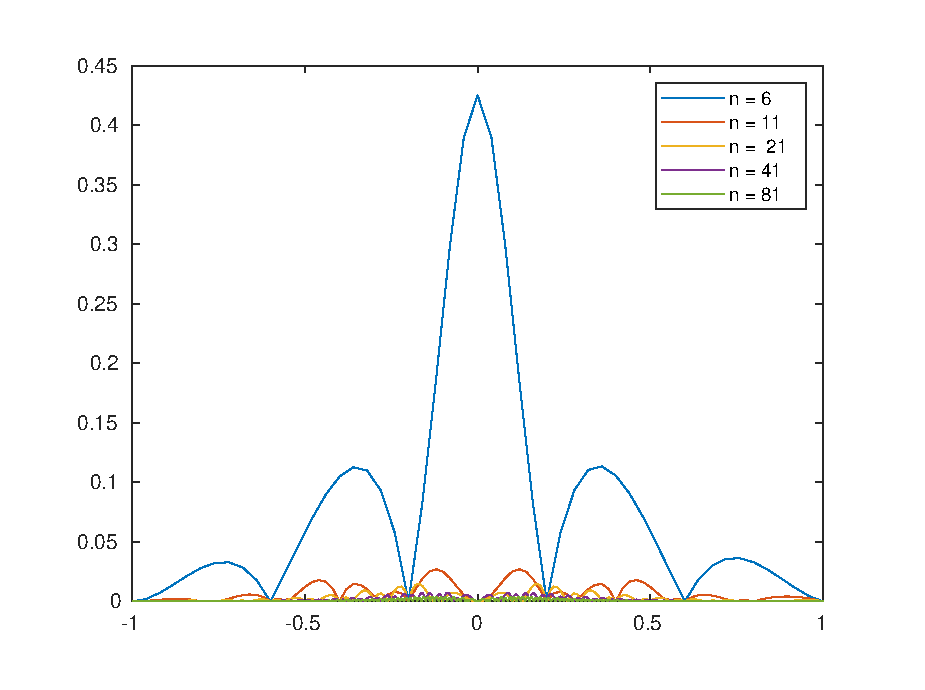
\includegraphics[width=7in]{error1.eps}
\caption{overall errors}
\end{figure}

\begin{figure}[h]
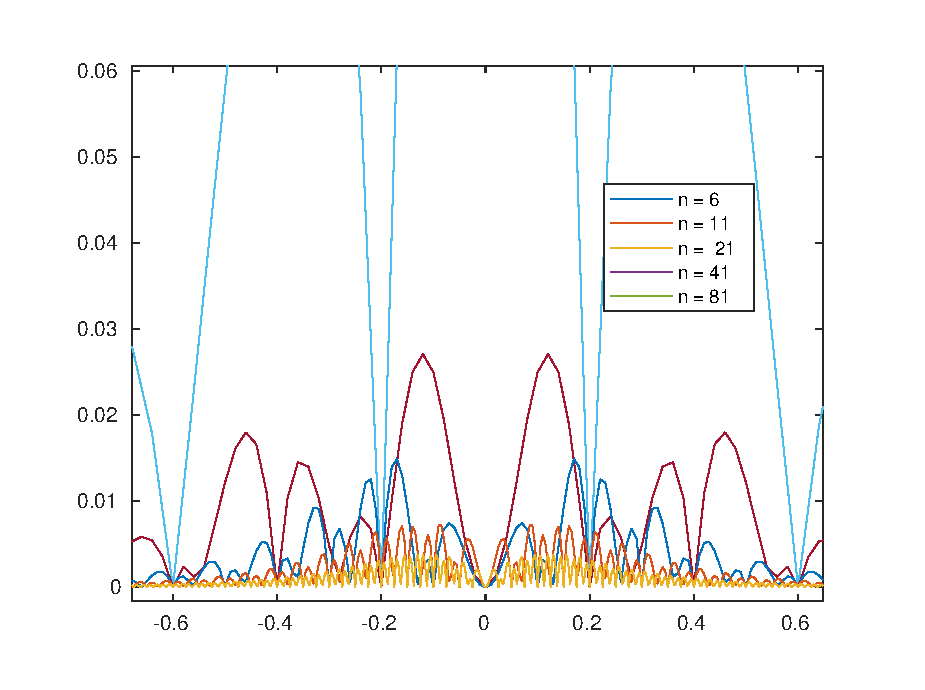
\includegraphics[width=7in]{error2.eps}
\caption{local errors}
\end{figure}

\end{document}
%%% Local Variables: 
%%% mode: latex
%%% TeX-master: t
%%% End: 
